\documentclass[a4paper,twoside]{article}

\usepackage{epsfig}
\usepackage{amssymb}
\usepackage{amstext}
\usepackage{amsmath}
\usepackage{amsthm}
\usepackage{multicol}
\usepackage{pslatex}
\usepackage{apalike}
\usepackage{SCITEPRESS}



\usepackage{subfig}
\usepackage{graphicx}
\usepackage{epstopdf}
\usepackage{flushend}
\usepackage{listings}
\usepackage{color}
\usepackage{multicol}
\usepackage{amsmath}

\usepackage{floatrow}


\lstset{breaklines=true}

\begin{document}

\title{MoBio - A mobile system for collecting electrophysiological data\subtitle{Preparation of Camera-Ready Contributions to SCITEPRESS Proceedings} }

\author{\authorname{Petr Je\v{z}ek\sup{1} and Roman Mou\v{c}ek\sup{1}}
\affiliation{\sup{1}New Technologies for the Information Society, 
              Department of Computer Science and Engineering,
              Faculty of Applied Sciences,
              University of  West Bohemia,
              Univerzitn\'{i} 8,
              306 14  Plze\v{n},
              Czech Republic}
\email{jezekp@ntis.zcu.cz, moucek@kiv.zcu.cz}
}   

\keywords{The paper must have at least one keyword. The text must be set to 9-point font size and without the use of bold or italic font style. For more than one keyword, please use a comma as a separator. Keywords must be titlecased.}

\abstract{The abstract should summarize the contents of the paper and should contain at least 70 and at most 200 words. The text must be set to 9-point font size.}

\onecolumn \maketitle \normalsize \vfill

\section{\uppercase{Introduction}}
\label{sec:introduction}

\noindent 
There are lot of factors affecting human health. Factors such as genetics, environmental influence or internal state of an individual cannot be easy measured. On the other hands there are factors as blood pressure, glucose level or heart rate that can be measured relatively easy, non-invasively by cheap sensors. For a long time electrophysiological experiments have been conducted in laboratories equipped by common desktop computers and non-transferable measuring devices. Fortunately situation is rapidly changing in these days. The one of reasons is increasing popularity of smart devices as phones or tablets. According to eMarketer \cite{emark} two billions of people will own a smart-phone in 2016. Simultaneously a lot of relatively cheap sensors for measurement of potentials from the human body is available on the market. These sensors often transfer data wirelessly, it means they can be easily read and processed by smart devices. This technical progress enables a particular shift of treatment from hospitals to home environments or facilitates collecting of data during outdoor activities. The obtained data can be used by two fundamental intersecting ways. 

The first assistive technology approach serves to stimulating, maintaining or improving functional capabilities of people with special needs including disabled people or aging population. Getting independence and self-sufficiency increases quality of life in general. 

The second approach is focused on sportsmen or actively living people. Measurements are based on a monitoring of persons when they are performing specific activities (e. g. running or long distance walking). The data are used to display the current status and a long term monitoring of the fitness level. 

We operate a complete equipped laboratory \cite{10.3389/fninf.2014.00020} for electrophysiology measurements. We are focused  mainly on Electroencephalography (EEG) and Event-related potentials (ERP). Except of the fixed laboratory we also operate a so-called mobile laboratory equipped by a set of laptops and portable measuring devices for performing experiments out of the laboratory. With advancing efforts for extension the laboratory to collect broader spectrum of data (e. g. blood pressure, Elektrocardiogram (EKG), glucose level, heart rate) we are proposing here a prototype of mobile client for collecting data from wireless devices. The client provides API for connecting to limited set of devices available on the market and enables synchronization with the remote storage.

\section{\uppercase{state of the art}}
\label{sec:state-of-the-art}

\noindent
According to \cite{Lowe2012242} applications using sensors can be divided into three categories. The first category Smart Phone Applications use either GPS or the
on-board kinematic sensors as the technologies of choice for monitoring exercise. The second category comprises of any system that uses a central controller
and an external sensor. The last category comes from image processing domain. It uses a combination of a computer screen and a camera. The camera monitors the exact movement and position of the entire body during exercise. The screen is used for the interaction with the user.

The first category represents application such as Endomondo or Runkeeper. The second category Nike+, miCoach, Garmin Heart Belt or Fora Active tonometer. The typical representative of third category is Microsoft Kinect.

While Microsoft Kinect is designed for the indoor use all other devices are designed mostly for the outdoor use. 

Available tools and sensors are usually designed for one specific activity. They are able to record only limited variety of data. In addition, due to proprietary structure they do not provide variability for integration with other systems. 

Moreower, neuroinformatics community identified problems with a long-term description, storage and management of experimental data/metadata \cite{CRCNS}. As a member of International Neuroinformatics Coordinating Facility (INCF) \cite{INCF} we are being developing a system for long term storage and management of EEG/ERP experiments - EEGBase \cite{ISI:000306821100004}. A mobile EEG-Base client \cite{10.3389/conf.fninf.2013.09.00046} is a supplementary Android tool that enables collecting experiments out of the laboratory and provides an on-line synchronization with EEGBase.


\section{\uppercase{Topologies and Data Transfer}}
\label{topology_data_transfer}

\noindent 
Sensors use different way to manipulate data. Some sensors have own display or internal memory for storing measured data these data can be transfered later. These devices usually provide a complete history of stored measurements. On the other hand devices such as heart rate meters do not have internal memory. Data can be transfered only in time of measurement. According to way of data distribution we defined three levels of topologies.

\begin{itemize}
 \item one-layer - The sensor is a stand-alone unit with controls, display and memory. Such a sensor is completely controlled without any connections to a remote system.   
 \item two-layers - Sensor only measures the data that send to a remote system. This system can be a common computer/laptop or a smart phone/watch etc. 
 \item three-layers - This topology adds a cloud service to the two-layers topology. Data are send to the server where they are analyzed. 
\end{itemize}

There are lot of sensors in one-layer topology including various glucometers, tonometers, stepcounters etc. These devices usually enables easy manipulation and do not require connection to any other system. Anyway the data are stored in proprietary storage that do not provide means for communication with other systems. Some sensors including heart rate belts or some step counters do not have own display. Data are usually displayed on a smart device screen. Because of limited performance of mobile devices only a basic data processing is provided. There is few exceptions as BlibCare tonometer equipped by WiFi. It enables a direct data transfer to a server using home network. 



\section{\uppercase{Mobile application prototype}}
\label{mobile_app_prototype}


\subsection{System Scope}
On the basis of difficulties with close-source dedicated devices we present a prototype of a mobile system that solves described problems by designing a mobile system relying on a standardized terminology describing sensors data. These terminology is implemented in an embedded database. The mobile system ensures the outdoor usage or the usage in environments without the Internet connectivity. When the client gets on-line the stored data are synchronized with EEGBase. Such a system aggregates data from various sensors in one place. Moreover, the data stored in a flexible data storage on the server can be used by human reared or processed by automatic readers.

\subsection{Format Selection}

\subsection{User Interface}

\subsection{Integration with EEGBase}

\section{Discussion}
\label{discussion}

\noindent

\section{Future Work}
\label{future-work}

\noindent


\begin{figure*}
% Use the relevant command to insert your figure file.
% For example, with the graphicx package use
\begin{tabular}{c}
\subfloat[List of available sensors]{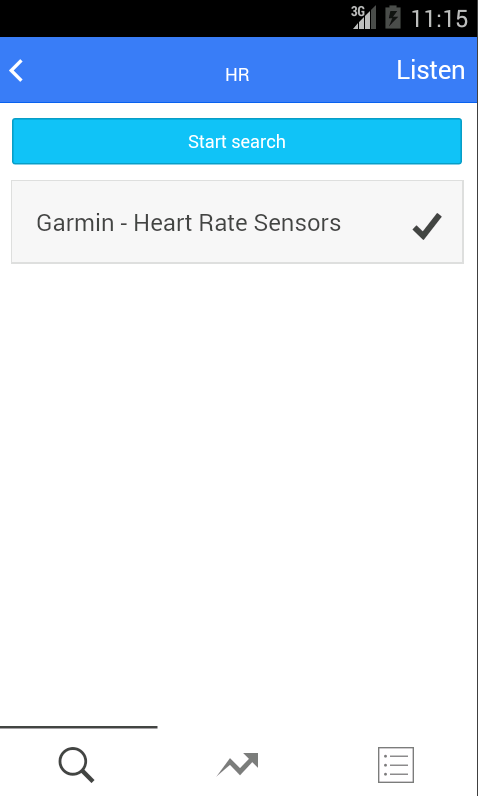
\includegraphics[width = 4cm, height=6.0cm]{Materials/Capture.PNG}\label{fig:capture_a}}
\hspace{10pt}\subfloat[Current heart rate]{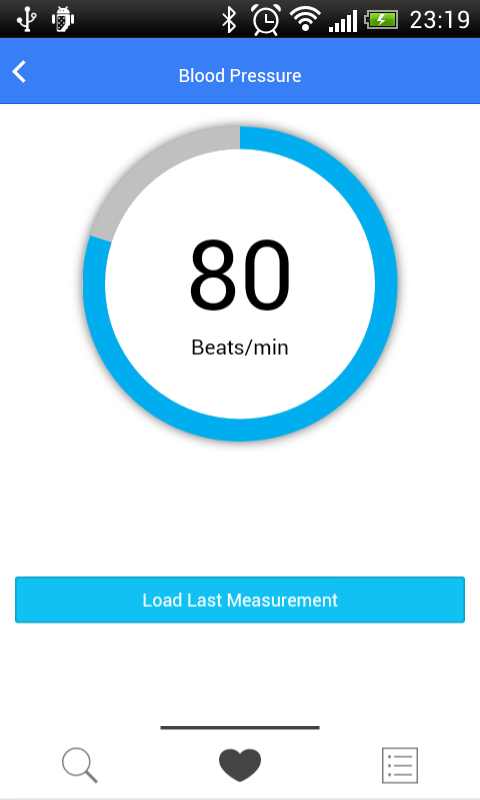
\includegraphics[width = 4cm, height=6.0cm]{Materials/Capture3.PNG}\label{fig:capture_b}}
\hspace{10pt}\subfloat[Long term heart rate]{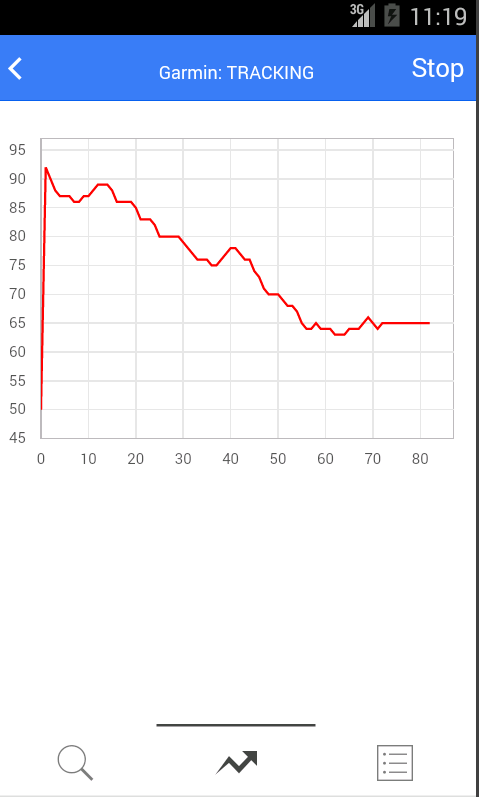
\includegraphics[width = 4cm, height=6.0cm]{Materials/Capture2.PNG}\label{fig:capture_c}}
\end{tabular}
% figure caption is below the figure
\caption{Mobile Application Preview}
\label{fig:mob_app_prev}
\end{figure*}   

\section{\uppercase{Conclusions}}
\label{sec:conclusion}

\noindent 

\section*{\uppercase{Acknowledgements}}

\noindent 
Will be added in CR version


\vfill
\bibliographystyle{apalike}
{\small
\bibliography{citations-healthinf-2016,frontiers,bibliography}


\vfill
\end{document}

